%%
%% This is file `sample-sigconf.tex',
%% generated with the docstrip utility.
%%
%% The original source files were:
%%
%% samples.dtx  (with options: `sigconf')
%% 
%% IMPORTANT NOTICE:
%% 
%% For the copyright see the source file.
%% 
%% Any modified versions of this file must be renamed
%% with new filenames distinct from sample-sigconf.tex.
%% 
%% For distribution of the original source see the terms
%% for copying and modification in the file samples.dtx.
%% 
%% This generated file may be distributed as long as the
%% original source files, as listed above, are part of the
%% same distribution. (The sources need not necessarily be
%% in the same archive or directory.)
%%
%%%% Proceedings format for most of ACM conferences (with the exceptions listed below) and all ICPS volumes.
\documentclass[sigconf,nonacm,11pt]{acmart}
%%%% As of March 2017, [siggraph] is no longer used. Please use sigconf (above) for SIGGRAPH conferences.

%%%% Proceedings format for SIGPLAN conferences 
% \documentclass[sigplan, anonymous, review]{acmart}

%%%% Proceedings format for SIGCHI conferences
% \documentclass[sigchi, review]{acmart}

%%%% To use the SIGCHI extended abstract template, please visit
% https://www.overleaf.com/read/zzzfqvkmrfzn

%%
%% \BibTeX command to typeset BibTeX logo in the docs
\AtBeginDocument{%
  \providecommand\BibTeX{{%
    \normalfont B\kern-0.5em{\scshape i\kern-0.25em b}\kern-0.8em\TeX}}}

\graphicspath{{fig/}{./}}

%%TC:ignore
%% Rights management information.  This information is sent to you
%% when you complete the rights form.  These commands have SAMPLE
%% values in them; it is your responsibility as an author to replace
%% the commands and values with those provided to you when you
%% complete the rights form.
\copyrightyear{2019}
\acmYear{2019}
\setcopyright{rightsretained}

%% These commands are for a PROCEEDINGS abstract or paper.
\acmConference{CSE6242}
\acmDOI{Data and Visual Analytics}
\acmISBN{}
\acmBooktitle{}
%%TC:endignore

%%
%% Submission ID.
%% Use this when submitting an article to a sponsored event. You'll
%% receive a unique submission ID from the organizers
%% of the event, and this ID should be used as the parameter to this command.
%%\acmSubmissionID{123-A56-BU3}

%%
%% The majority of ACM publications use numbered citations and
%% references.  The command \citestyle{authoryear} switches to the
%% "author year" style.
%%
%% If you are preparing content for an event
%% sponsored by ACM SIGGRAPH, you must use the "author year" style of
%% citations and references.
%% Uncommenting
%% the next command will enable that style.
%%\citestyle{acmauthoryear}

%%
%% end of the preamble, start of the body of the document source.
\begin{document}

%%
%% The "title" command has an optional parameter,
%% allowing the author to define a "short title" to be used in page headers.
\title{Evaluating Household Debt}

%%
%% The "author" command and its associated commands are used to define
%% the authors and their affiliations.
%% Of note is the shared affiliation of the first two authors, and the
%% "authornote" and "authornotemark" commands
%% used to denote shared contribution to the research.

%%TC:ignore
\author{George I. Kaveladze, Jason I. Chavez, John H. Tang, Khwala A. Abdulgader, Oluwagbemiga M. Adeosun}
\email{{gkaveladze3, jchavez8, jtang338, kabdulgader3, oadeosun7}@gatech.edu}
\affiliation{%
}

% \author{John Smith}
% \affiliation{\institution{The Th{\o}rv{\"a}ld Group}}
% \email{jsmith@affiliation.org}

% \author{Julius P. Kumquat}
% \affiliation{\institution{The Kumquat Consortium}}
% \email{jpkumquat@consortium.net}
%%TC:endignore

%%
%% By default, the full list of authors will be used in the page
%% headers. Often, this list is too long, and will overlap
%% other information printed in the page headers. This command allows
%% the author to define a more concise list
%% of authors' names for this purpose.
%%TC:ignore
%%\renewcommand{\shortauthors}{Tobin, et al.}
%%TC:endignore

%%
%% The abstract is a short summary of the work to be presented in the
%% article.
\begin{abstract}

The ability to accurately predict economic expansion or contraction is shown to be heavily reliant on household debt.  The correlation between economic downturns and high household debt levels is high, with household debt to GDP ratios having slightly higher predictive power.  Our household debt dashboard will provide users with the ability to observe the effects that changes in economic factors has on household debt and economic health, by proxy.  This approach will differentiate itself by predicting a factor that plays a large role in economic health, rather than attempting to predict economic health as a whole, allowing the model to account for more nuanced prediction factors.\vspace{-0.5em}

\end{abstract}

%%
%% The code below is generated by the tool at http://dl.acm.org/ccs.cfm.
%% Please copy and paste the code instead of the example below.
%%
%%TC:ignore
% \begin{CCSXML}
% <ccs2012>
%  <concept>
%   <concept_id>10010520.10010553.10010562</concept_id>
%   <concept_desc>Computer systems organization~Embedded systems</concept_desc>
%   <concept_significance>500</concept_significance>
%  </concept>
%  <concept>
%   <concept_id>10010520.10010575.10010755</concept_id>
%   <concept_desc>Computer systems organization~Redundancy</concept_desc>
%   <concept_significance>300</concept_significance>
%  </concept>
%  <concept>
%   <concept_id>10010520.10010553.10010554</concept_id>
%   <concept_desc>Computer systems organization~Robotics</concept_desc>
%   <concept_significance>100</concept_significance>
%  </concept>
%  <concept>
%   <concept_id>10003033.10003083.10003095</concept_id>
%   <concept_desc>Networks~Network reliability</concept_desc>
%   <concept_significance>100</concept_significance>
%  </concept>
% </ccs2012>
% \end{CCSXML}

% \ccsdesc[500]{Computer systems organization~Embedded systems}
% \ccsdesc[300]{Computer systems organization~Redundancy}
% \ccsdesc{Computer systems organization~Robotics}
% \ccsdesc[100]{Networks~Network reliability}

%%
%% Keywords. The author(s) should pick words that accurately describe
%% the work being presented. Separate the keywords with commas.
\keywords{Datasets, Household Debt, Economic Visualization, Household Debt to GDP Ratio, GDP Ratio, Interest Rate\vspace{-0.79em}}
%%TC:endignore

%% A "teaser" image appears between the author and affiliation
%% information and the body of the document, and typically spans the
%% page.
% \begin{teaserfigure}
%   \includegraphics[width=\textwidth]{sampleteaser}
%   \caption{Seattle Mariners at Spring Training, 2010.}
%   \Description{Enjoying the baseball game from the third-base
%   seats. Ichiro Suzuki preparing to bat.}
%   \label{fig:teaser}
% \end{teaserfigure}
%%
%% This command processes the author and affiliation and title
%% information and builds the first part of the formatted document.
%%TC:ignore
\maketitle
%%TC:endignore
\section{Introduction}

The field of macroeconomics has produced a wide variety of research into the predictability of economic expansion and contraction. Interest in this research field has increased over the years with many recent recessions providing a swath of data that can be analyzed and evaluated to determine the level of predictive power. The Great Recession of 2008, for instance, highlighted a set of factors that could be used to predict economic fluctuations, including recessions and market corrections.  Household debt, for example, was shown to have a negative impact on the GDP despite providing a short-term stimulus\cite{Kim2016}.  Accurately predicting this value could provide insights into of economic fluctuations and financial instability associated with government policies and consumer spending.  Research conducted by Zabai\cite{Zabai2017} has indicated that there is a direct correlation between economic health and household debt. Our goal for this project is to provide an interactive dashboard that allows users to observe correlations between household debt and other economic factors, along with predicting household debt given user-determined values for factors like Federal Interest Rates and yields on 10-year US bonds.\\
Since a large and rapid increase in household debt points to economic slowdown\cite{Mian2018}, this information can help users understand the impact their spending habits have. Similarly, the ability to adjust values and see outcomes could help legislators better understand the impact their policies have on the economy\cite{Garber2018}.\vspace{-1em}

%%\section{Key Features}

%% The Household Debt Dashboard will allow users to observe and quickly discern correlative associations between household debt and major economic factors.  Users will have the opportunity to adjust certain factors and observe the consequences of these values through the output of our Machine Learning algorithm that displays the predicted household debt.  This information will be coupled with GDP levels to enhance the user's understanding of the macroeconomic effects their proposals have.  Lastly, our solution will provide a containerized solution that allows interested parties to load the development environment necessary to create new models and visualization.\vspace{-1em}

\section{Problem Definition}

When a decline in the economic activity has been observed for multiple consecutive months a recession is to be expected in the United States. This directly destabilizes households, small businesses, and large corporations; even when US policy makers utilize stimulus packages to mitigate long-term consequences; such as a spike in the unemployment percentages and defaults on mortgages. Recessions have been observed to follow a business cycle. The ability to predict when the next economic downturn will occur allows corporations and US policy makers to properly plan and prevent a greater negative impact to the economy. As previous research has indicated there is a strong correlation between economic downturns and a high household debt, our dashboard will allow users to observe the effects that changes in economic factors have on household debt and economic health, by proxy.  Users will have the opportunity to adjust certain factors and observe the consequences of these values through the output of our Machine Learning algorithm that displays the predicted household debt. \vspace{-1em}

\section{Survey}

Our dashboard will leverage several studies performed on the correlative effects of household debt and economic downturns.\\
\textbf{Studying The Great Recession}\\
Many studies have been conducted to better understand the factors that lead to the 2008 recession, including Chakrabarti et al.'s evaluation of household debt and savings during the recession\cite{Chakrabarti2015}, Nyman et al.'s Machine Learning approach to understanding the great recession\cite{Nyman2018}, and Mian et al.'s observation of household leverage and the recession\cite{Mian2010}.  All articles show the high correlation between economic downturns and increased household debt. We've used these article to back our belief in the utility of household debt predictions and will leverage to evaluate variable importance.\\
\textbf{Macroeconomic effects of Household Debt}\\
General evaluations of the macroeconomic effects have been outlined in great detail in papers like Alter et al.'s global perspective on household debt effects\cite{Alter2018}, Friedman's theory of the consumption function\cite{Friedman1957}, Kim's empirical analysis of the effects of household debt\cite{Kim2016}, Lombardi et al.'s evaluation of the real effects of household debt\cite{Lombardi2017}, Mian et al.'s observations on household debt and worldwide business cycles\cite{Mian2015}\cite{Mian2018}, and Filardo's assessment on  the reliability of prediction models\cite{Filardo1999}. Each of these articles provide a backing for the global reach our proposed predictions can have, and provide a solid background on which correlations should receive particular attention. We'll expand this information by including more concentrated variables that relate specifically to household debt.\\
\textbf{Policy Impacts on Economies and Household Debt}\\
If the provided proof of the relation between household debt and economic health have provided justification for our dashboard, studies on legislative effects provide motivation for creating the dashboard.  Garber et al.'s study of Brazil's 2014 recession\cite{Garber2018} and Guggenheim Investments' look into the effects rate cuts will continue to have in the US economic health\cite{Guggenheim2019} provide a basis for which variables our dashboard will allow users to adjust.\\
\textbf{Current State of Debt}\\
A major push to produce our dashboard has come from research that reveal household debt is steadily climbing.  From Li's evaluation on the economics of student loans\cite{Li2013}, to Mian et al.'s study on the household leverage crisis\cite{Mian2011} and Zabai's assessment on recent household debt developments\cite{Zabai2017}, we've come to realize how much household debt continues to grow.  Leveraging this information, we hope to reveal what factors might be leading to this troubling trend.

%%\section{Risks, Rewards, and Cost}

%%\subsection{Risks}

%%We need as many input variables added in our model in the short time frame of the project.  For each input variable we need a large dataset to maximize the predictive power of the machine learning algorithm. The risk of influencing major decisions based on a poor prediction carries a heavy consequence.  While our models might show favorable statistics (e.g. low R2 and Mean Squared Error values), there is always the risk that our models either overfit the data or are biased towards a certain outcome.  Since mitigation strategies often include increasing training data observations, we also run the risk of not having a diverse enough set of training data to model against. 

%%\subsection{Rewards}

%The payoff of a model that accurately predicts household debt and presents it in an intuitive dashboard is huge. As Mian et al. observed, "the larger the increase in household leverage prior to the recession, the more severe the subsequent recession."\cite{Mian2018}.  Providing this information could encourage lawmakers to move beyond hypothetical outcomes and observe data driven predictions of economic responses.\vspace{-1em}

%\subsection{Costs}
%We will use open source data and software so the cost will be minimal other than human capital.  Depending on the availability and arrangements of Georgia Tech cloud based resources, the cost to host our solution would be the only concern.
\section{Proposed Method}
The following sections outline the methodology we have taken to produce our application:.\vspace{-0.5em}

\subsection{Dashboard}
The Household Debt dashboard will provide a multi-faceted approach to understanding the effects that various factors have on how citizen's borrowing practices.  This will be accomplished by, first, allowing users to observe visualizations that convey the relations between a subset of factors and household debt.  As household debt increases have been shown to be directly correlated with economic health\cite{Mian2015}, these visualizations will allow users to better understand the contributions that this debt has on a macroeconomic level and help curb the significant growth in household debt\cite{Alter2018}.\\
Additionally, users will have the ability to adjust the values associated with these highly correlative factors and observe the resulting household debt predictions.  Our predictions will be presented both textually and graphically as we explore visualizations that demonstrate the prediction's relation to GDP.\vspace{-0.5em}

\subsection{Predictions}

In order to provide significant predictions, we will gather data from a variety of sources and evaluate variable importance for predicting household debt. As of 03/26/20, the team has collected ~25 various economic data variables and completed a correlation analysis using R.  While other models have been created using the random forest algorithm\cite{Nyman2018}, we will compare model scores from multiple models.\vspace{-0.5em}

\subsection{Technologies}

Our dashboard front end will be created using D3.js visualizations. The application's user interface is a responsive single page application (SPA) based on AngularJS and Bootstrap. We'll containerize our solution using Docker to allow users to use our cleaned data for their own exploration. Our website will be hosted on Heroku and has a Node.js back-end. We are utilizing SQLite for data storage locally, as we are not deploying this to our website. Machine Learning models will be created using Azure ML Studio, providing an API for the front end. \vspace{-0.5em}


\subsection{Innovations}

Our dashboard includes the following innovative approaches; firstly, based on our extensive research, there is a limited amount of models focusing on predicting household debt only; even though it is a strong indicator to the economic health of the United States. Many financial institutions produce economic models using household debt as a primary variable, therefore we are going to focus on this specific variable rather than predict the larger economy. Secondly, we are trying to account for negative rates by researching whether we should include global negative rates into our model or negative real rates. This will all our model to include data that is typically not used in United States recession models as the data is unavailable, but provides a complete view to an economic downturn. Lastly, we are streamlining our dashboard by providing an API of our machine learning model to the front-end and having a Node.js back-end while containerizing our solution using Docker.\vspace{-0.5em}

\section{Experiments and Evaluation}
In order to validate our methodology when creating our household debt dashboard, we have complied a list of steps that we will be reviewing throughout our process. These steps are outlined as follows; firstly, we have collected a large amount of data-sets to determine which data elements will provide the highest prediction power as we believe this will allow us to have the best prediction performance. Secondly, we will be evaluating multiple machine learning algorithms to ensure we are utilizing the most suitable methodology when predicting household debt. Thirdly, we have included a user functionality feature as we believe allowing the user to select various data elements will provide a greater understanding of the factors that impact household debt. Fourthly, we have been researching various economic dashboard visualizations to ensure we compartmentalize the information in an intuitive manner for the user. Lastly, we believe our front-end and back-end methodology is stream-lined as stated in the innovations section above. 

We have evaluated the first step as we've completed our correlation analysis in R and are currently in process of selecting the variables with the highest prediction power; such as Auto Dealer Sales which has a correlation coefficient of 0.578 and GDP which has correlation coefficient of 0.471. We are currently in process of evaluating which machine learning algorithm to utilize through Azure ML Studio and are finalizing which visualizations to display on the dashboard as we have already created the front and back-end of the application (see Figure 5.1).

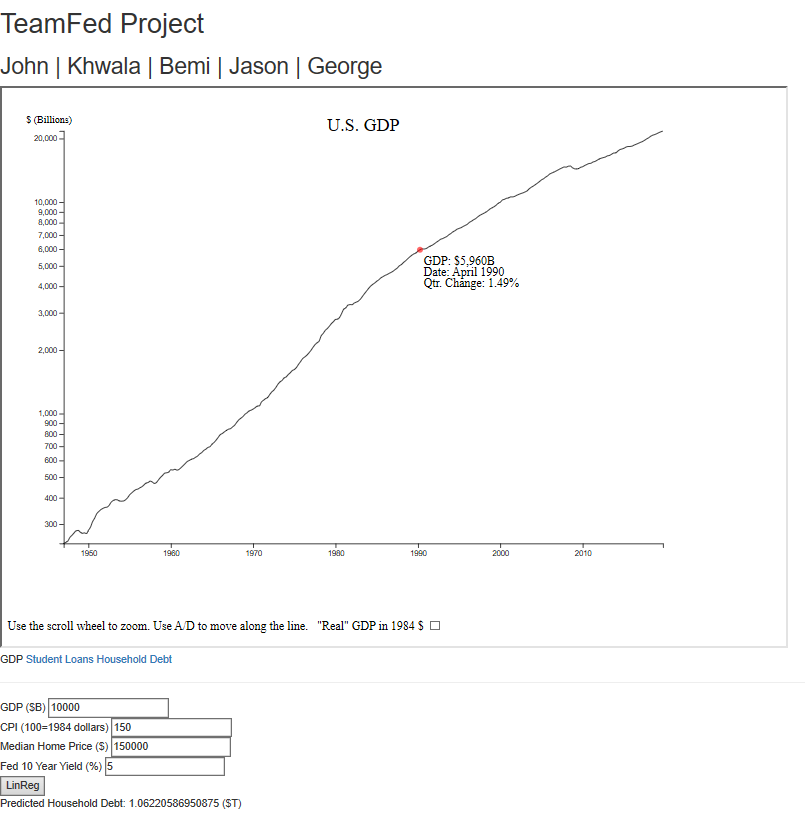
\includegraphics[scale = 0.59]{teamfed2.PNG}
Figure 5.1 displays our preliminary application using raw data as we are finalizing variable selection and our machine learning algorithm \vspace{-0.5em}


\section{Plan of Activities}

We plan on achieving success by following the plan below:\vspace{0.07em}
\begin{center}
    \begin{tabular}{||c|c||}
    \hline
    Activity & Completion Date (02/28)\\
    \hline\hline
    Collect Data & 03/07\\
    Variable Exploration & 03/14\\
    Clean Data & 03/21\\
    Variable Selection & 03/21\\
    Progress Report & 03/27\\
    ML Algorithm Developed & 03/31\\
    Front-end Setup & 03/31 \\
    Back-end Setup & 03/31 \\
    Final Report & 03/27\\
    \hline
    \end{tabular}
\end{center}

\begin{center}
    \begin{tabular}{||c|c||}
    \hline
    Activity & Completion Date (03/27)\\
    \hline\hline
    Collect Data & 03/07\\
    Variable Exploration & 03/20\\
    Clean Data & 03/21\\
    Variable Selection & 03/27\\
    Progress Report & 03/27\\
    ML Algorithm Developed & 04/03\\
    Front-end Setup & 04/03\\
    Back-end Setup & 03/31\\
    Final Report & 04/05\\
    \hline
    \end{tabular}
\end{center}

\textbf{All group members have continued to contribute a similar amount of effort.} The following activities will be continued to be led by these teammates: Data Collection: John and Khwala; Variable Exploration: George; Data Cleansing: John and Jason; Variable Selection: Jason and Khwala; ML Algorithm: Jason; Front-end Set Up: Bemi and George; Back-end Set Up: Bemi; Progress and Final Report: Khwala. As a note, it is expected that all teammates will continue to support and provide input for each activity.

%\section{Related Work}

%Our dashboard will leverage several studies performed on the correlative effects of household debt and economic downturns.\\
%\textbf{Studying The Great Recession}\\
%Many studies have been conducted to better understand the factors that lead to the 2008 recession, including Chakrabarti et al.'s evaluation of household debt and savings during the recession\cite{Chakrabarti2015}, Nyman et al.'s Machine Learning approach to understanding the great recession\cite{Nyman2018}, and Mian et al.'s observation of household leverage and the recession\cite{Mian2010}.  All articles show the high correlation between economic downturns and increased household debt, which we've used to back our belief in the utility of household debt predictions and will leverage to evaluate variable importance.\\
%\textbf{Macroeconomic effects of Household Debt}\\
%General evaluations of the macroeconomic effects have been outlined in great detail in papers like Alter et al.'s global perspective on household debt effects\cite{Alter2018}, Friedman's theory of the consumption function\cite{Friedman1957}, Kim's empirical analysis of the effects of household debt\cite{Kim2016}, Lombardi et al.'s evaluation of the real effects of household debt\cite{Lombardi2017}, Mian et al.'s observations on household debt and worldwide business cycles\cite{Mian2015}\cite{Mian2018}, and Filardo's assessment on  the reliability of prediction models\cite{Filardo1999}. Each of these articles provide a backing for the global reach our proposed predictions can have, and provide a solid background on which correlations should receive particular attention. We'll expand this information by including more concentrated variables that relate specifically to household debt.\\
%\textbf{Policy Impacts on Economies and Household Debt}\\
%If the provided proof of the relation between household debt and economic health have provided justification for our dashboard, studies on legislative effects provide motivation for creating the dashboard.  Garber et al.'s study of Brazil's 2014 recession\cite{Garber2018} and Guggenheim Investments' look into the effects rate cuts will continue to have in the US economic health\cite{Guggenheim2019} provide a basis for which variables our dashboard will allow users to adjust.\\
%\textbf{Current State of Debt}\\
%A major push to produce our dashboard has come from research that reveal household debt is steadily climbing.  From Li's evaluation on the economics of student loans\cite{Li2013}, to Mian et al.'s study on the household leverage crisis\cite{Mian2011} and Zabai's assessment on recent household debt developments\cite{Zabai2017}, we've come to realize how much household debt continues to grow.  Leveraging this information, we hope to reveal what factors might be leading to this troubling trend.

\bibliographystyle{ACM-Reference-Format}
\bibliography{reference}

%%
%% If your work has an appendix, this is the place to put it.
\appendix

% \section{Research Methods}

% \subsection{Part One}

% Lorem ipsum dolor sit amet, consectetur adipiscing elit. Morbi
% malesuada, quam in pulvinar varius, metus nunc fermentum urna, id
% sollicitudin purus odio sit amet enim. Aliquam ullamcorper eu ipsum
% vel mollis. Curabitur quis dictum nisl. Phasellus vel semper risus, et
% lacinia dolor. Integer ultricies commodo sem nec semper.

% \subsection{Part Two}

% Etiam commodo feugiat nisl pulvinar pellentesque. Etiam auctor sodales
% ligula, non varius nibh pulvinar semper. Suspendisse nec lectus non
% ipsum convallis congue hendrerit vitae sapien. Donec at laoreet
% eros. Vivamus non purus placerat, scelerisque diam eu, cursus
% ante. Etiam aliquam tortor auctor efficitur mattis.

% \section{Online Resources}

% Nam id fermentum dui. Suspendisse sagittis tortor a nulla mollis, in
% pulvinar ex pretium. Sed interdum orci quis metus euismod, et sagittis
% enim maximus. Vestibulum gravida massa ut felis suscipit
% congue. Quisque mattis elit a risus ultrices commodo venenatis eget
% dui. Etiam sagittis eleifend elementum.

% Nam interdum magna at lectus dignissim, ac dignissim lorem
% rhoncus. Maecenas eu arcu ac neque placerat aliquam. Nunc pulvinar
% massa et mattis lacinia.
\end{document}
\endinput
%%
%% End of file `sample-sigconf.tex'.
